\documentclass[12pt]{article}
\usepackage[english]{babel}
\usepackage[utf8x]{inputenc}
\usepackage{fullpage}
\usepackage{graphicx}
\usepackage[version=3]{mhchem} 
\usepackage{siunitx} 
\usepackage{graphicx}
\usepackage{natbib} 
\usepackage{amsmath} 


\usepackage{listings}
\usepackage{color}

\title{Laboratory work nr. 2  \\Analyzing of sorting algorithms\\ } % Title

\author{\textsc{Bîrcu} \textsc{Maxim}} % Author name

\date{\today} % Date for the report

\definecolor{mygreen}{rgb}{0,0.6,0}
\definecolor{mygray}{rgb}{0.5,0.5,0.5}
\definecolor{mymauve}{rgb}{0.58,0,0.82}

\lstset{ %
  backgroundcolor=\color{white},   % choose the background color
  basicstyle=\footnotesize,        % size of fonts used for the code
  breaklines=true,                 % automatic line breaking only at whitespace
  captionpos=b,                    % sets the caption-position to bottom
  commentstyle=\color{mygreen},    % comment style
  escapeinside={\%*}{*)},          % if you want to add LaTeX within your code
  keywordstyle=\color{blue},       % keyword style
  stringstyle=\color{mymauve},     % string literal style
}

\begin{document}


\maketitle % Insert the title, author and date

\begin{center}
\begin{tabular}{l r}

Student: & Bîrcu Maxim \\ % Partner names
Instructor: & Cojanu Irina % Instructor/supervisor

\end{tabular}
\end{center}


\subsection*{Work purpose}
\subparagraph*{
\\1. Studing of 3 sorting algorithms \\
2. Implementation of those sorting algorithms\\
3. Results analyzing }

\newpage
\section*{Results}

\subparagraph*{I've studied three methods of sorting (bubble sort, merge sort and quick sort) for different rows of names arranged in random order, and calculated the number of iterations for each of these methods to the same string, the results I have scored in a table.
}

\section{Random inputs}

\begin{figure}[h!]
  \centering
    {%
      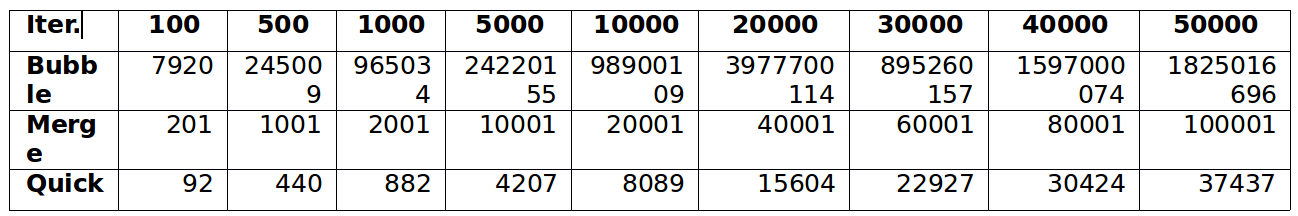
\includegraphics[width=0.5\textwidth]{1}}
\end{figure}

\subsection*{
For better understanding of the results I've placed them on a graph.
}


\begin{figure}[h!]
  \centering
    {%
      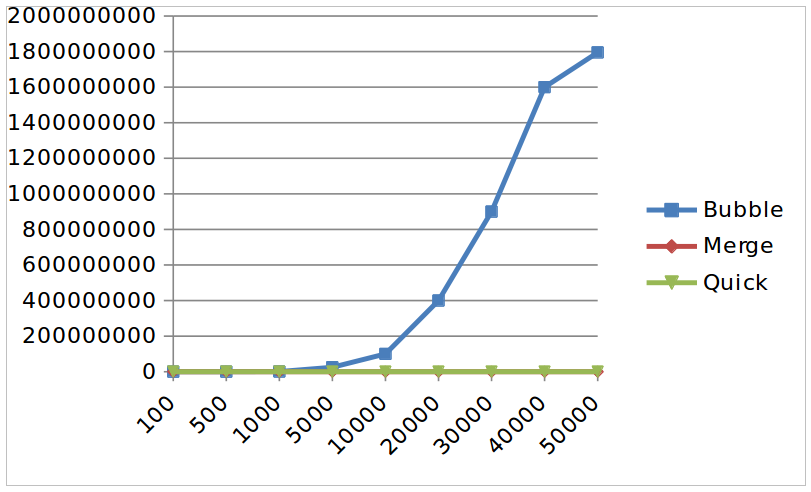
\includegraphics[width=0.5\textwidth]{8}}
\end{figure}

\subparagraph*{
We denote that sorting method with most iterations is Bubble sort which was expected. And the increasing of the number of iterations for merge an quick sort are pretty the same. So the most inefficient algorithm is Bubble sort.
}




\newpage
\section{Favorable case}

\begin{figure}[h!]
  \centering
    {%
      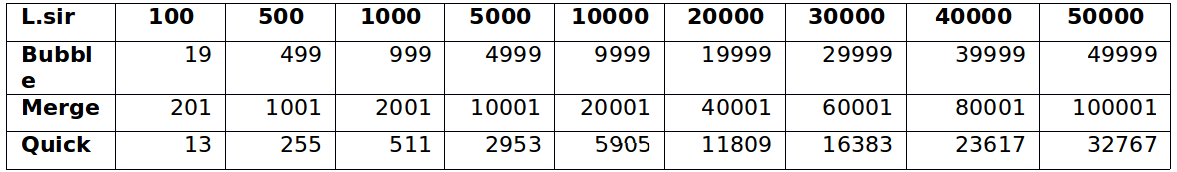
\includegraphics[width=0.5\textwidth]{5}}
\end{figure}

\subsection*{
For better understanding of the results I've placed them on a graph.
}

\begin{figure}[h!]
  \centering
    {%
      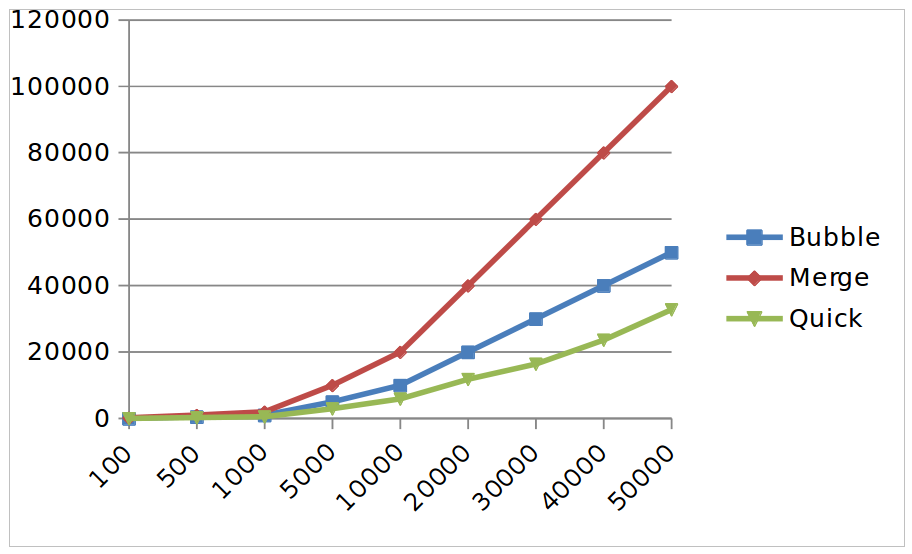
\includegraphics[width=0.5\textwidth]{6}}
\end{figure}

\subparagraph*{
	We can observe that in the favorable case all algorithms has uniform increasing , the faster increasing is for merge sort , and also we can observe that the number of iterations of merge sort algorithm do not depend of the case because in random case we have the same results for this algorithm. Also if we compare Quick and Bubble sort we can observe a small difference and make the conclusion that Quick sort is quite faster than Bubble and Merge sort.
}


\newpage
\section{Unfavorable case}

\begin{figure}[h!]
  \centering
    {%
      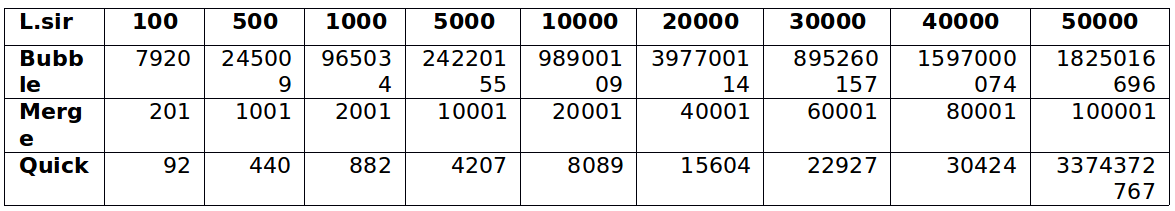
\includegraphics[width=0.5\textwidth]{7}}
\end{figure}

\subsection*{
For better understanding of the results I've placed them on a graph.
}

\begin{figure}[h!]
  \centering
    {%
      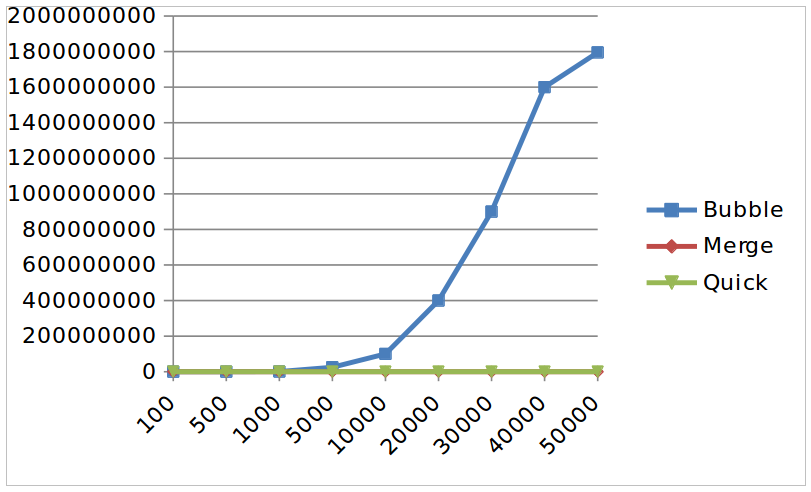
\includegraphics[width=0.5\textwidth]{8}}
\end{figure}

\subparagraph*{
Here we can observe from the graph that Bubble sort has an abnormal increasing and therefore it is inefficient and we should study the last 2 methods in another graph without bubble sort. 
}

\newpage
\begin{figure}[h!]
  \centering
    {%
      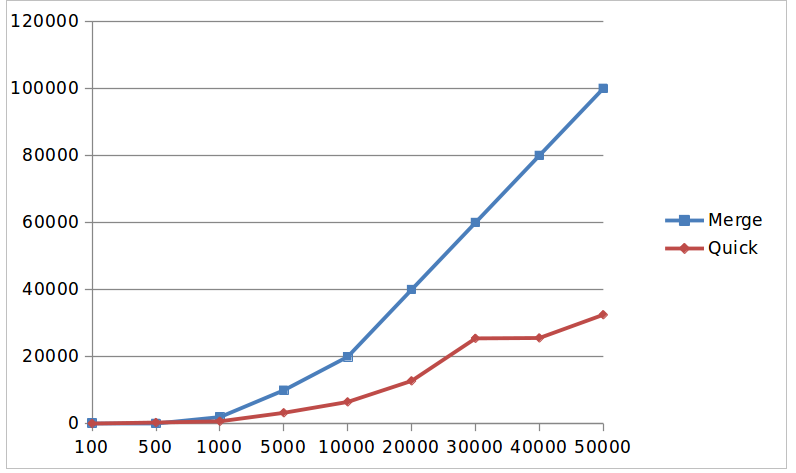
\includegraphics[width=0.5\textwidth]{4}}
\end{figure}

\subparagraph*{Now we can see the difference between the number of iterations of the merge sort an quick sort algorithms. We can observe that Merge sort has a uniform increasing of iterations number in comparison with Quick sort but Quick sort has a slower increasing than Merge sort.}

\section{Conclusion:}
\subparagraph*{After all research and algorithms comparison I've observed that the efficiency of the algorithm in some cases depends on the input size and form which means the random case when the list is sorted randomly , the favorable case when the list is sorted ascendant and the unfavorable case when the list is sorted descendant. Also I observed that in all 3 cases the quick sort algorithm was the most efficient.
About Merge an Bubble sort I can say that if we have to chose one of this 2 algorithms our choosing will depend on the problem. So if we will have to check if a list is sorted than the most efficient algorithm will be Bubble sort but if we should sort a descendant sorted list probably merge sort will be a better choosing than Bubble sort.}
\end{document}